\definecolor{HallowGreen}{RGB}{50,110,30}
\providecommand{\iRef}[1]{{\tiny\color{HallowGreen} $[$#1$]$}}

\author[Tanjona Rabemananjara]{}
\institute{University of Milan}

\subsection{PDF compression}

\begin{frame}{A new methodology with GANs}
	S. Carrazza, J. Cruz-Martinez, \underline{T. Rabemananjara} \\
	\textbf{\textcolor{HallowGreen}{\underline{Goal}:}} Provide a smaller set of MC 
	replicas that best represents the Probability Distribution of a given PDF set 
	with large samples.
	\vspace*{-0.1cm}	
	\begin{center}
	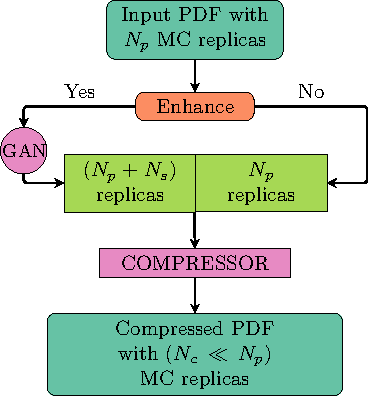
\includegraphics[height=.7\textheight]{./gan_compressor/imgs/pygans.pdf}
	\end{center}
\end{frame}

\begin{frame}{Compression results}
	\underline{Standard vs. GAN-Enhanced Compressor}:
	\begin{center}
		\textcolor{red}{\textbf{\underline{SETUP}:}} ($N_p=1000 + N_s=2000$) 
		$\longrightarrow$ $N_c$
	\end{center}
	\begin{columns}[T] 
	\begin{column}{.5\textwidth}
	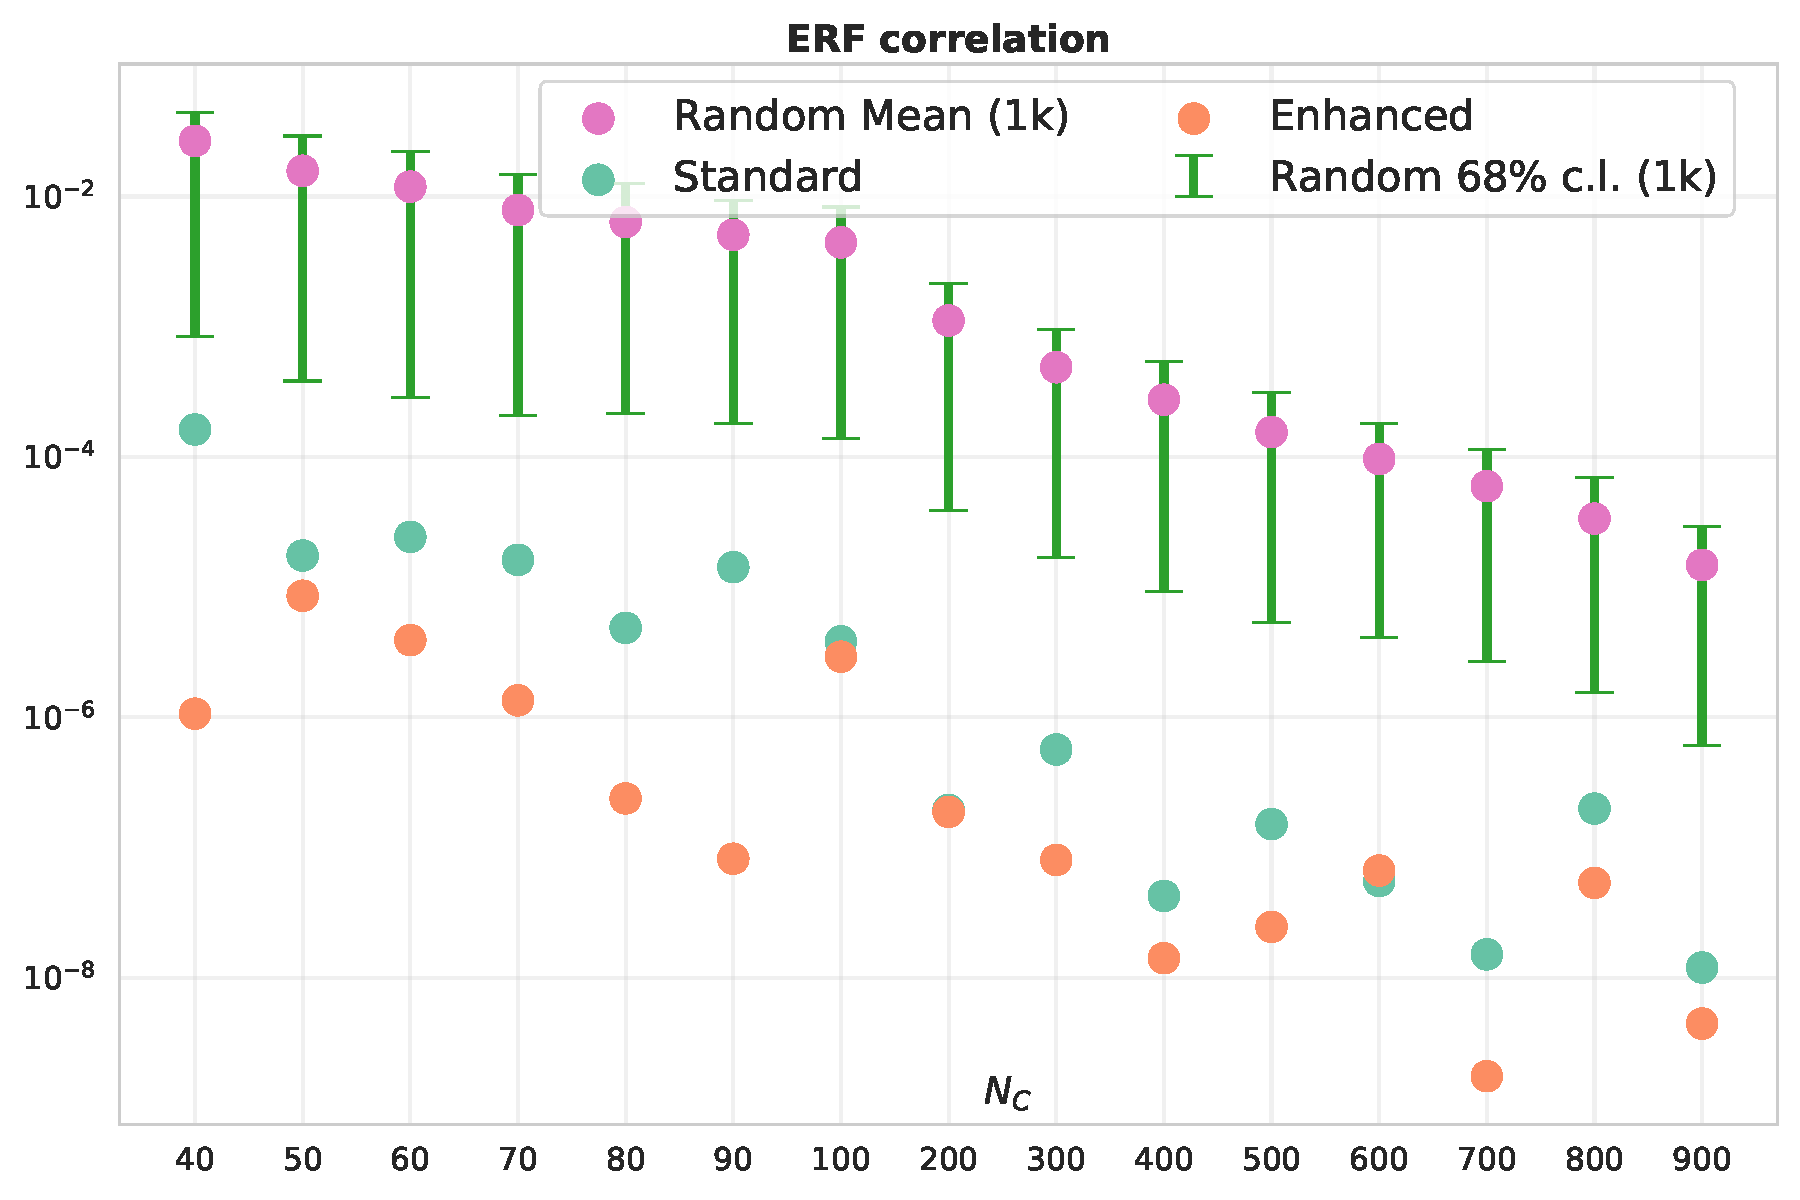
\includegraphics[width=\linewidth]{./gan_compressor/imgs/erf-validation.pdf}
	\end{column}
	\begin{column}{.5\textwidth}	
	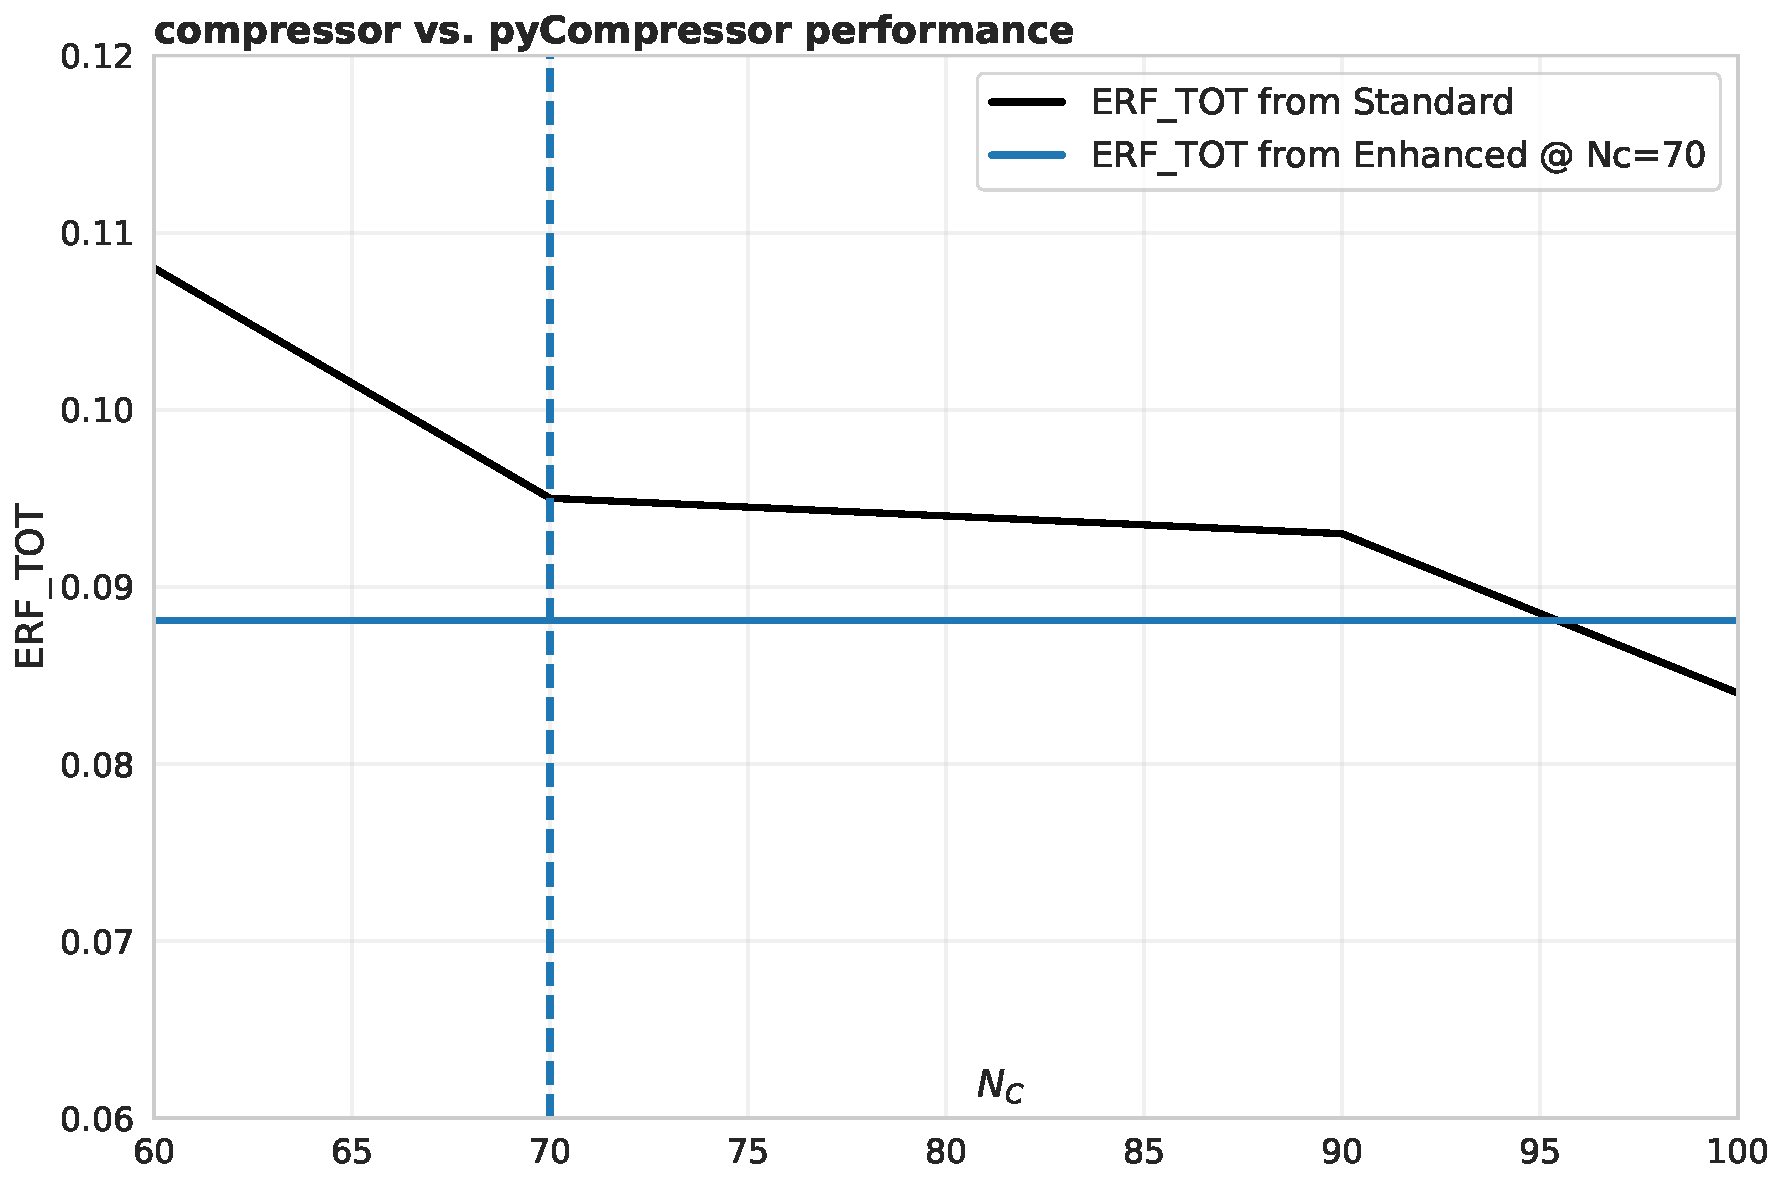
\includegraphics[width=\linewidth]{./gan_compressor/imgs/performance.pdf}
	\end{column}
	\end{columns}
	\begin{center}
	\begin{tcolorbox}[width=9.5cm, halign=center, colframe=HallowGreen]
		$N_c (\text{GAN-Enhanced})=70 \sim N_c (\text{Standard})=95$
	\end{tcolorbox}
	\end{center}
\end{frame}
